\documentclass[12pt]{article}
\usepackage[papersize={8cm,12cm},margin={.5cm,.5cm}]{geometry}
\usepackage{common}
\usepackage{amssymb}
\begin{document}
\begin{problem}
  \item[9.] 已知圖(五)的直角柱中,每一個底面都是正三角形,面積均為 $a$;每一個側面都是矩形,面積均為 $b$。則此角柱的表面積應為下列何者?
  \begin{figure}[ht]
    \centering
    \vspace*{-1ex}
    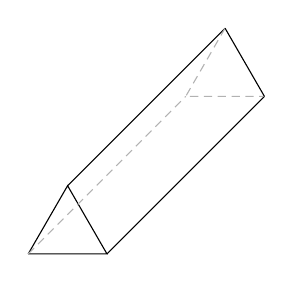
\begin{tikzpicture}
      \draw (0,0) -- (1,0) -- (.5,.866) -- (0,0);
      \draw[densely dashed,black!30] (0,0) -- (2,2);
      \draw (1,0) -- (3,2);
      \draw (.5,.866) -- (2.5,2.866);
      \draw[densely dashed,black!30] (2.5,2.866) -- (2,2) -- (3,2);
      \draw (3,2) -- (2.5,2.866);
    \end{tikzpicture}
    \vspace*{-1ex}
    \caption*{圖(五)}
    \vspace*{-2ex}
  \end{figure}
  \begin{choices}
    \item $a + b$
    \item $a + 2b$
    \item $2a + 2b$
    \item $2a + 3b$
  \end{choices}
\end{problem}
\end{document}
